\documentclass[twocolumn]{article}  
\usepackage[top = 1.5cm, bottom = 1.5cm, left = 1.0cm, right = 1.0cm]{geometry}  
\usepackage{graphicx}
\usepackage{amsmath}  
\usepackage{gensymb}
\usepackage{ multirow }
\usepackage[inline]{enumitem}
\setlength{\columnseprule}{0.4pt}
\setlength{\columnsep}{3em}
\makeatletter
% This command ignores the optional argument for itemize and enumerate lists
\newcommand{\inlineitem}[1][]{%
\ifnum\enit@type=\tw@
    {\descriptionlabel{#1}}
  \hspace{\labelsep}%
\else
  \ifnum\enit@type=\z@
       \refstepcounter{\@listctr}\fi
    \quad\@itemlabel\hspace{\labelsep}%
\fi}
\makeatother

\title{DL Assignment-01}
\date{}
\author{Rohan Anil Muskawad\\2020A8PS1798P}
\begin{document}  
\maketitle

\section{[Page 83 -to- 85]}

\begin{enumerate}
        
        \item Group which contains the maximum number of student is
            \begin{enumerate}
                \item 130-140 \inlineitem 140-150
                \item 150-160 \inlineitem 160-170
                
            \end{enumerate}
                \textbf{Direction(2):}Study the histogram of weight distribution of different men and answer question based on it
            \begin{flushright}
                \textbf{[SSC CGL 2013]}
            \end{flushright}

            \begin{center}
                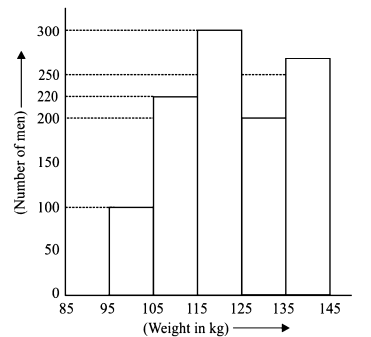
\includegraphics[scale=0.4]{pic1.png}
            \end{center}
            
        \item Average number of men per interval who participated in the survey is
            \begin{enumerate}
                \item 180
                \inlineitem 194
                \item 200
                \inlineitem 214
            \end{enumerate}

            \textbf{Direction(3-4):}The histogram shows the marks of 50 students in an examination. Examine the diagram and answer the question \hfill\textbf{[SSC MTF 2013]}
            
            \begin{center}
                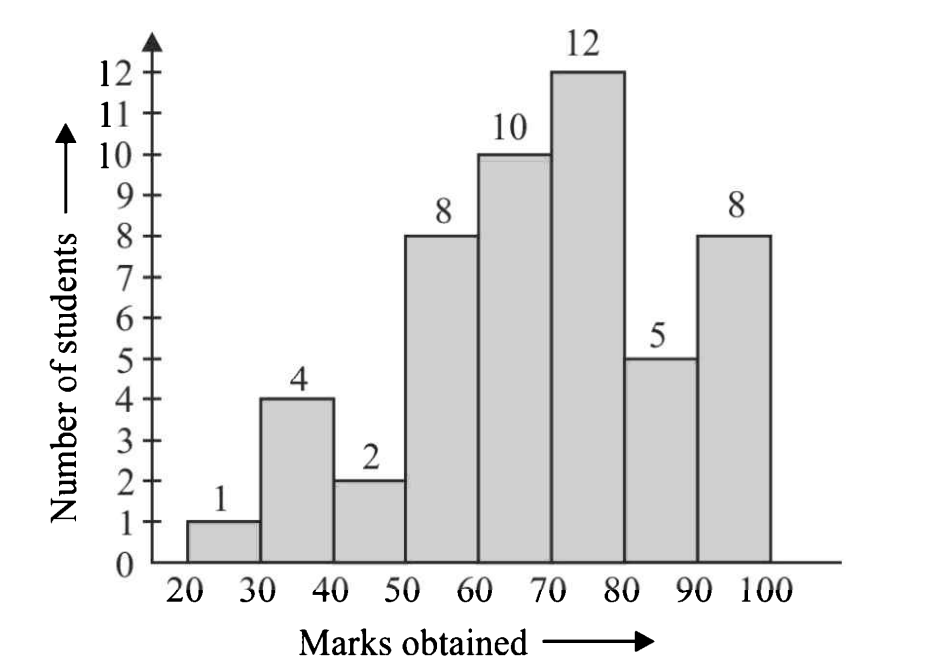
\includegraphics[scale=0.4]{pic2.png}
            \end{center}

        \item How many students obtained more than 39 but below 60?
            \begin{enumerate}
                \item 6
                \inlineitem 8
                \item 10
                \inlineitem 12
            \end{enumerate}

        \item What percent of students did obtain marks above 60\%
        \begin{enumerate}
            \item 60\%
            \inlineitem 70\%
            \item 75\%
            \inlineitem 80\%
        \end{enumerate}
        \textbf{Direction(5-6):}Study the graphs carefully and answer the qeustion \hfill\textbf{[SSC CGL 2013]}
        \begin{center}
            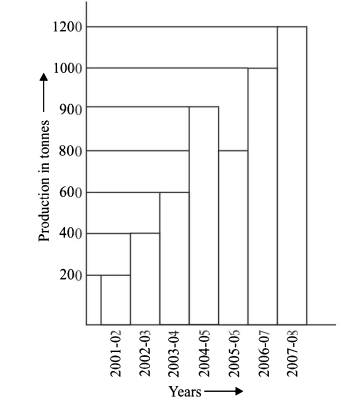
\includegraphics[scale=0.4]{pic3.png}
        \end{center}
        \item The production in 2006-07 in comparison to the production in 2002-03 increased by
            \begin{enumerate}
                \item 110\%
                \inlineitem 120\%
                \item 125\%
                \inlineitem 150\%
            \end{enumerate}
        \item The production decreased from 2004-05 to 2005-06 by
        \begin{enumerate}
            \item $\displaystyle 8\frac{1}{9}$\%
            \inlineitem $\displaystyle 9\frac{1}{9}$\%
            \item $\displaystyle 10\frac{1}{9}$\%
            \inlineitem $\displaystyle 11\frac{1}{9}$\%
        \end{enumerate}
        \item The year in which production increase the lowest as compared to the previous year is
            \begin{enumerate}
                \item 2003-04
                \inlineitem 2004-05
                \item 2006-07
                \inlineitem 2007-08
            \end{enumerate}
            \item The production from 2003-04 to 2007-08 increased by
            \begin{enumerate}
                \item 50\%
                \inlineitem 75\%
                \item 100\%
                \inlineitem 125\%
            \end{enumerate}
            \textbf{Direction(9-11):}Study the following frequency polygon and answer the questions \hfill\textbf{[SSC CGL 2015]}
            \begin{center}
                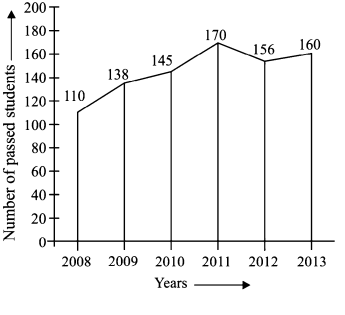
\includegraphics[scale=0.4]{pic4.png}
            \end{center}
            \item The average of passed students in the years 2008, 2009, 2012 approximately is
            \begin{enumerate}
                \item 134.34
                \inlineitem 134.41
                \item 134.56
                \inlineitem 134.67
            \end{enumerate}
            \item The increase in percentage of passed students from 2008 to 2011 approximately is
            \begin{enumerate}
                \item 50.5\%
                \inlineitem 53.05\%
                \item 54.5\%
                \inlineitem 55\%
            \end{enumerate}
            \item The decrease in percentage of passed students from 2011 to 20122 approximately is
            \begin{enumerate}
                \item 8.22\%
                \inlineitem 8.24\%
                \item 8.25\%
                \inlineitem 8.27\%
            \end{enumerate}
            \textbf{Direction(12-13):}Study the following data and answer the questions \hfill\textbf{[SSC CGL 2015]}
            \begin{tabular}{ |l|l|l|l|l| }\hline
                IQ Score & 80-90 & 90-100 & 100-110 & 110-120 \\\hline 
                Number & 6 & 9 & 16 & 13 \\\hline 
            \end{tabular}
            \item Number of students who IQ score is 140 is
            \begin{enumerate}
                \item 0
                \inlineitem 1
                \item 2
                \inlineitem Undeterminable from given data
            \end{enumerate}
            \item The number of students whose IQ score is 100 and more is
            \begin{enumerate}
                \item 29
                \inlineitem 35
                \item 36
                \inlineitem 46
            \end{enumerate}
            \newpage
\end{enumerate}
\pagebreak
\begin{enumerate} 
    \item A circle is inscribed in a trianlge ABC. It touches the sides AB,BC and AC at the points R,P and Q respectively. If AQ=4.5cm PC=5.5cm and BR=6cm, then the perimeter of the triangle ABC is:
        \begin{enumerate}
            \item 30.5cm \inlineitem 28cm
            \item 32cm \inlineitem 26.5cm
        \end{enumerate}
        \item The table shows the production of different types of cars (in thousands)\\
        \begin{tabular}{ |l|l|l|l|l|l| }\hline
            Cars/Years & 2012 & 2013 & 2014 & 2015 & 2016 \\\hline 
            A & 30 & 35 & 48 & 45 & 56 \\\hline 
            B & 42 & 48 & 40 & 38 & 56 \\\hline
            C & 48 & 36 & 38 & 35 & 44 \\\hline  
            D & 51 & 24 & 30 & 46 & 54 \\\hline
            E & 20 & 42 & 40 & 35 & 43 \\\hline  
        \end{tabular}\\
        If the data related to the prodcution of cars of type E is represented by a pie chart, the the central angle of the sector representing the data of production of cars in 2013 will be:
        \begin{enumerate}
            \item 102\degree \inlineitem 84\degree
            \item 70\degree \inlineitem 80\degree
        \end{enumerate}
        \item A truck covers a distance of 384km at a certain speed. If the speed is decreased by 16km/h, it will take 2 hours more to cover the same distance. 75\% of its original speed(in km/h) is:
            \begin{enumerate}
                \item 45
                \inlineitem 54
                \item 48
                \inlineitem 42
            \end{enumerate}
        \item The ratio of the ages of A and B, four years ago, was 4:5. Eight years from now, the ratio of the ages of A and B will be 11:13. What is the saum of their present ages?
        \begin{enumerate}
            \item 80 years
            \inlineitem 96 years
            \item 72 years
            \inlineitem 76 years
        \end{enumerate}
        \item In $\triangle$ ABC , F and E are the points on sides AB and AC, respectively, such the FE $\parallel$ BC divides the triangle in two parts of equal area. If AD $\perp$  BC and AD intersects FE at G, the GD:AG =?
            \begin{enumerate}
                \item $\sqrt{2}:1$
                \inlineitem $(\sqrt{2}-1):1$
                \item $2\sqrt{2}:1$
                \inlineitem $(\sqrt{2}+1):1$
            \end{enumerate}
        \item If $4-2sin^{2}\theta - 5cos\theta =0$ $0\degree < \theta < 90 \degree$, then the valye of $sin\theta + tan\theta $ is:
        \begin{enumerate}
            \item $ \frac{3\sqrt{2}}{2}$
            \inlineitem  $ \frac{3\sqrt{3}}{2}$
            \item $3\sqrt{2}$
            \inlineitem $2\sqrt{3}$
        \end{enumerate}
        \item The table shows the production of different types of cars (in thousands)\\
        \begin{tabular}{ |l|l|l|l|l|l| }\hline
            Cars/Years & 2012 & 2013 & 2014 & 2015 & 2016 \\\hline 
            A & 30 & 35 & 48 & 45 & 56 \\\hline 
            B & 42 & 48 & 40 & 38 & 56 \\\hline
            C & 48 & 36 & 38 & 35 & 44 \\\hline  
            D & 51 & 24 & 30 & 46 & 54 \\\hline
            E & 20 & 42 & 40 & 35 & 43 \\\hline  
        \end{tabular}\\
        What is the raito of the total production of cars of type A in 2014 and type C in 2013 taken together to the total production of cars of type B in 2016 and type E in 2015 taken together?
        \begin{enumerate}
            \item 12:13 \inlineitem 11:12
            \item 10:11 \inlineitem 12:11
        \end{enumerate}
        \item If decreasing 120 by x\% gives the same result as increase 40 by x\% then x\% of 210 is what percent less than (x+20)\% of 180?
        \begin{enumerate}
            \item $\displaystyle 33\frac{1}{3}$
            \inlineitem 18
            \item $\displaystyle 16\frac{2}{3}$
            \inlineitem 20
        \end{enumerate}
        \item If $(5\sqrt{5}x^{3}-81\sqrt{3}y^{3})\div(\sqrt{5}x-3\sqrt{3}y)=(Ax^{2}+By^{2}+Cxy)$ then the value of $(6A+B-\sqrt{15}C)$
        \begin{enumerate}
            \item 10
            \inlineitem 9
            \item 15
            \inlineitem 12
        \end{enumerate}
        \item If a nine-digit number 958x3678y is divisible by 72, then the valye of(4x-3y) is:
        \begin{enumerate}
            \item 5
            \inlineitem 4
            \item 6
            \inlineitem 3
        \end{enumerate}
        \item If $sin\theta = \frac{P^{2}-1}{P^{2}+1}$, then $cos\theta$ is equal to:
        \begin{enumerate}
            \item $\frac{2P}{P^{2}+1}$
            \inlineitem $\frac{P}{P^{2}-1}$
            \item $\frac{P}{P^{2}+1}$
            \inlineitem $\frac{2P}{P^{2}-1}$
        \end{enumerate}
        \item The ratio of the efficiencies of A,B and C is 2:5:3. Working together, they can complete a work in 27 days. B and C together can complete $\frac{4}{9}$th part of that work in:
        \begin{enumerate}
            \item 27days
            \inlineitem 15days
            \item 17$\frac{1}{7}$ days
            \inlineitem 24days
        \end{enumerate}
\end{enumerate}
\end{document}
